\documentclass[12pt,]{book}
\usepackage{lmodern}
\usepackage{setspace}
\setstretch{1.5}
\usepackage{amssymb,amsmath}
\usepackage{ifxetex,ifluatex}
\usepackage{fixltx2e} % provides \textsubscript
\ifnum 0\ifxetex 1\fi\ifluatex 1\fi=0 % if pdftex
  \usepackage[T1]{fontenc}
  \usepackage[utf8]{inputenc}
\else % if luatex or xelatex
  \ifxetex
    \usepackage{mathspec}
  \else
    \usepackage{fontspec}
  \fi
  \defaultfontfeatures{Ligatures=TeX,Scale=MatchLowercase}
\fi
% use upquote if available, for straight quotes in verbatim environments
\IfFileExists{upquote.sty}{\usepackage{upquote}}{}
% use microtype if available
\IfFileExists{microtype.sty}{%
\usepackage{microtype}
\UseMicrotypeSet[protrusion]{basicmath} % disable protrusion for tt fonts
}{}
\usepackage[margin=1in]{geometry}
\usepackage{hyperref}
\hypersetup{unicode=true,
            pdftitle={Characterization of the MHC I immunopeptidome of HaCaT cells},
            pdfauthor={Alistair Bailey},
            pdfborder={0 0 0},
            breaklinks=true}
\urlstyle{same}  % don't use monospace font for urls
\usepackage{natbib}
\bibliographystyle{apalike}
\usepackage{longtable,booktabs}
\usepackage{graphicx,grffile}
\makeatletter
\def\maxwidth{\ifdim\Gin@nat@width>\linewidth\linewidth\else\Gin@nat@width\fi}
\def\maxheight{\ifdim\Gin@nat@height>\textheight\textheight\else\Gin@nat@height\fi}
\makeatother
% Scale images if necessary, so that they will not overflow the page
% margins by default, and it is still possible to overwrite the defaults
% using explicit options in \includegraphics[width, height, ...]{}
\setkeys{Gin}{width=\maxwidth,height=\maxheight,keepaspectratio}
\IfFileExists{parskip.sty}{%
\usepackage{parskip}
}{% else
\setlength{\parindent}{0pt}
\setlength{\parskip}{6pt plus 2pt minus 1pt}
}
\setlength{\emergencystretch}{3em}  % prevent overfull lines
\providecommand{\tightlist}{%
  \setlength{\itemsep}{0pt}\setlength{\parskip}{0pt}}
\setcounter{secnumdepth}{5}
% Redefines (sub)paragraphs to behave more like sections
\ifx\paragraph\undefined\else
\let\oldparagraph\paragraph
\renewcommand{\paragraph}[1]{\oldparagraph{#1}\mbox{}}
\fi
\ifx\subparagraph\undefined\else
\let\oldsubparagraph\subparagraph
\renewcommand{\subparagraph}[1]{\oldsubparagraph{#1}\mbox{}}
\fi

%%% Use protect on footnotes to avoid problems with footnotes in titles
\let\rmarkdownfootnote\footnote%
\def\footnote{\protect\rmarkdownfootnote}

%%% Change title format to be more compact
\usepackage{titling}

% Create subtitle command for use in maketitle
\newcommand{\subtitle}[1]{
  \posttitle{
    \begin{center}\large#1\end{center}
    }
}

\setlength{\droptitle}{-2em}
  \title{Characterization of the MHC I immunopeptidome of HaCaT cells}
  \pretitle{\vspace{\droptitle}\centering\huge}
  \posttitle{\par}
  \author{Alistair Bailey}
  \preauthor{\centering\large\emph}
  \postauthor{\par}
  \predate{\centering\large\emph}
  \postdate{\par}
  \date{May 09 2018}


% Preamble
\usepackage[none]{hyphenat}
\usepackage[default,osfigures,scale=0.95]{opensans} % Open sans font
\usepackage[T1]{fontenc} % Use 8-bit encoding that has 256 glyphs
\usepackage{lettrine} % The lettrine is the first enlarged letter at the beginning of the text
\raggedbottom 
\usepackage{makeidx} % These lines add bibliography to TOC
\makeindex
\usepackage[nottoc]{tocbibind}
\renewcommand{\bibname}{References} % Rename biblography as References

\begin{document}
\maketitle

{
\setcounter{tocdepth}{1}
\tableofcontents
}
\listoftables
\listoffigures
\chapter*{Summary}\label{summary}
\addcontentsline{toc}{chapter}{Summary}

This report details objective 1 of the ImmunoSense project:
Characterization of the MHC I immunopeptidome of HaCaT cells \(\pm\)
DNCB.

The key findings are:

\begin{itemize}
\tightlist
\item
  The identification of 7611 unique peptides under control conditions.
\item
  The identification of 6687 unique peptides under DNCB treatment
  conditions.
\item
  9mer peptides represent around 55\% of the total peptidome across all
  six replicates.
\item
  60\% of unique peptides are shared between treatment and control
  peptidomes, with 25\% and 14\% of peptides seen only in control and
  treatment peptidomes respectively.
\item
  Two DNCB modified peptides were identified in two biological
  replicates (four technical replicates).
\item
  One of the modified peptides derived from a Keratin, type I
  cytoskeletal 13 protein
  (\href{https://www.uniprot.org/uniprot/P13646}{P13646})
\item
  The second modified peptide derived from the active site of
  Glutathione S-transferase omega-1
  (\href{https://www.uniprot.org/uniprot/P78417}{P78417})
\end{itemize}

\chapter{Introduction}\label{introduction}

This report details objective 1 of the ImmunoSense project:
Characterization of the MHC I immunopeptidome of HaCaT cells
\citep{boukamp1988} \(\pm\) DNCB. The HaCaT cell line is a spontaneously
transformed keratinocyte line.

Here we seek to capture class I major histocompatibility complex
molecules (MHC I) presented on the surface of cells. MHC I sample the
intracellular proteome in the form of short peptides, predominantly 9
amino acids in length. The collective name for the peptides presented is
the immunopeptidome. For a recent summary of MHC I antigen processing
and presentation see \citep{hateren2017a}.

We used HaCaT cells to test two non-exclusive hypotheses:

\begin{itemize}
\item
  Sensitiser-modified peptides presented by MHC I directly stimulate the
  immune system.
\item
  Sensitiser modification of proteins alters the MHC I presented
  repertoire of peptides.
\end{itemize}

2,4-Dinitrochlorobenzene (DNCB) is our model sensitiser. In cell lysates
DNCB modifies approximately 0.12\% Lys, 0.03\% Cys and \textless{}
0.03\% Tyr, His and Arg \citep{parkinson2018}.



\begin{figure}

{\centering \includegraphics[width=0.15\linewidth]{img/DNCB} 

}

\caption{The structure of 2,4-Dinitrochlorobenzene (DNCB).}\label{fig:dncb}
\end{figure}

For an overview of immunopeptidomics goals and challenges see this short
article: \citep{caron2017}.

Figure \ref{fig:workflow} shows the immunopeptidome workflow used in the
generation of this work.



\begin{figure}

{\centering 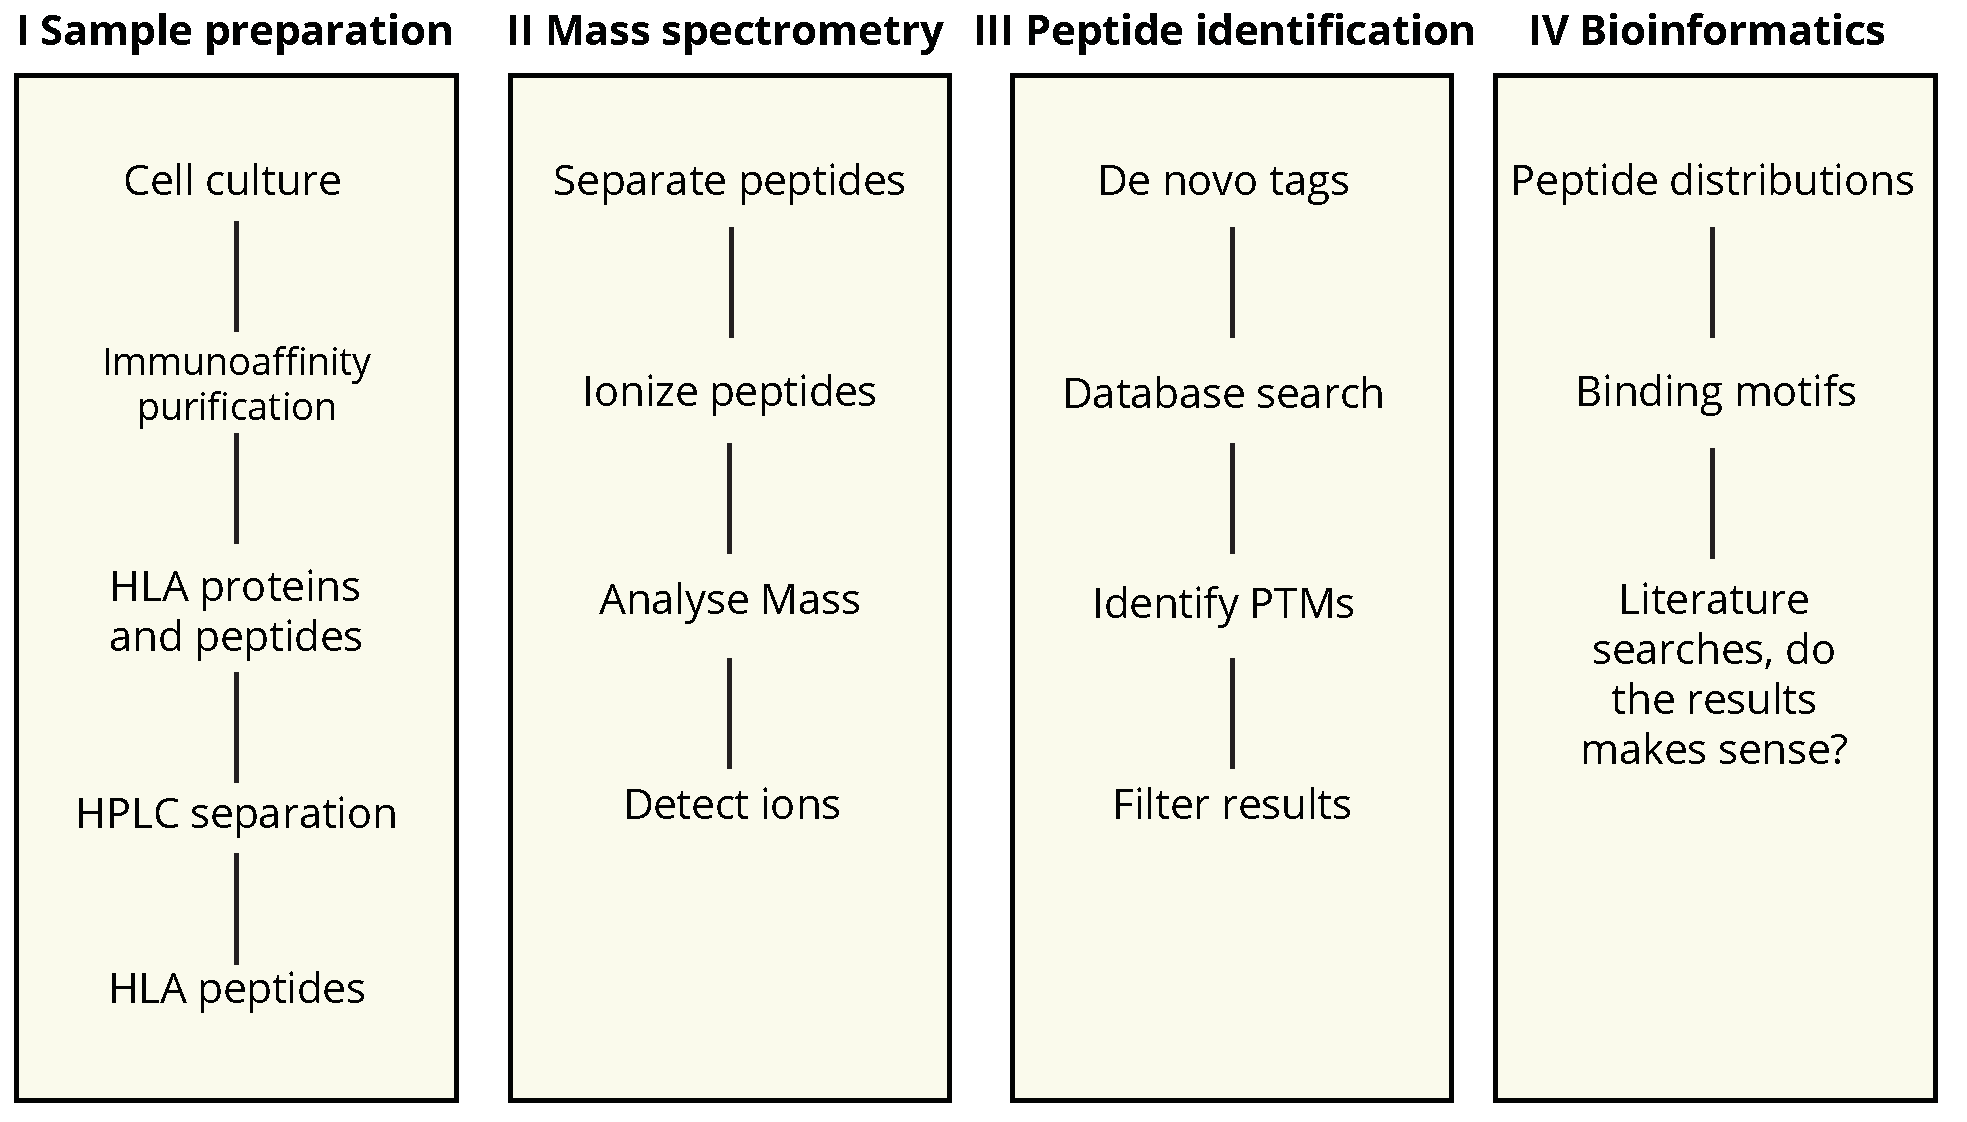
\includegraphics{img/mass_spec_summary} 

}

\caption{The immunopeptidome workflow.}\label{fig:workflow}
\end{figure}

The following sections detail the
\protect\hyperlink{methods}{methodology},
\protect\hyperlink{peptidome-size-and-proportions}{summary tables,
histograms and venn diagrams},
\protect\hyperlink{peptide-binding-motifs}{biochemical properties of the
peptidomes} and \protect\hyperlink{dncb-modifications}{properties of
DNCB modified peptides}.

\hypertarget{methods}{\chapter{Methods}\label{methods}}

\hypertarget{cell-culture}{\section{Cell culture}\label{cell-culture}}

HaCaT cells \citep{boukamp1988} purchased from
\href{http://clsgmbh.de/}{Cell lines service} were cultured in DMEM
medium supplemented with 4.5g/L glucose and 2mM L-glutamine and 10\%
fetal bovine serum.

For each replicate two populations were grown to 500 x
10\textsuperscript{6} cells each, and then the medium changed to
DMEM/F-12 without serum. One population was used for the control and the
other population treated with a 10 \(\mu\)M 2,4-Dinitrochlorobenzene
(DNCB) mixture of DNCB and DNCB-D\textsubscript{3} for 24 hours. Cells
were harvested with 0.25\% Trypsin-EDTA and then washed with DPBS and
pelleted prior to freezing and storage at -80\(^\circ\)C.

Three biological replicates of control and treatment pellets were
cultured, these were then split in half to create six technical
replicates:

\begin{itemize}
\tightlist
\item
  1A and 1B
\item
  2A and 2B
\item
  3A and 3B
\end{itemize}

\section{HLA typing of HaCaT cells}\label{hla-typing-of-hacat-cells}

DNA extraction performed with QIAGEN DNAeasy kit under the supervision
of Dr.~Emma Reeves, and typing done by Southampton General Hospital
tissue typing unit.

Confirmation of these results was made using genomics analysis using
publicly available datasets and
\href{https://ccb.jhu.edu/software/hisat2/index.shtml}{HISAT2}
\citep{kim2015}.

Together this yielded HLA types:

\begin{itemize}
\tightlist
\item
  Homozygous HLA-A*31:01
\item
  HLA-B*40:01, HLA-B*51:01
\item
  HLA-C*03, HLA-C*15
\end{itemize}

There is uncertainty of the C alleles beyond two digit identification.

The literature had indicated that HaCaTs carried HLA-A*02
\citep{lemaitre2004}, but our results disconfirm this observation.

\section{Immunoaffinity purification and HPLC
fractionation}\label{immunoaffinity-purification-and-hplc-fractionation}

Cells were lysed in a buffer of 20 mM Tris-HCL (pH 8.0), 150 mM NaCl,
0.5\% IGEPAL, 0.25\% Sodium deoxycholate, 1 mM EDTA, 0.2 mM
Iodoacetamide and protease inhibitors at 4\(^\circ\)C on a roller for 30
minutes.

Cell nuclei were removed by centrifugation at 2,000g for 10 minutes. The
remaining lysate was then clarified by centrifugation at 15,000g (13,000
rpm) for 1 hour.

The lysate was then added to a tube containing pan-MHC I binding
antibody W6/32 crosslinked to Protein A sepahrose beads at a
concentration of 2 mg antibody per mL of beads and incubated on a roller
at 4\(^\circ\)C for 2 hours.

The lysate and beads were then transferred to a column for washing and
elution of the MHC I molecules using 5 mL 10\% acetic acid, denaturing
the MHC I molecules into a heavy chain, \(\beta\)\textsubscript{2}m and
peptide mixture.

The eluate was then dried in a speed-vac evaporator and re-suspended in
500 \(\mu\)L of 0.1\% TFA/1\% acetonitrile prior to injection into the
high performance liquid chromatography (HPLC) system.

A Thermo UltiMate 3000 system using a Chromolith HighResolution RP-18
endcapped 100-4.6 HPLC column were used to separate and collect the
peptides for mass spectrometry analysis. 0.5 mL peptide fractions were
collected over 8 minutes. These fractions were pooled as odd and even
fractions and then dried in a speed-vac evaporator.

These fractions were then re-suspended in 20 \(\mu\)L of 1\% Formic acid
and split into four samples, two odd and two even, for mass spectrometry
analysis.

\section{Mass spectrometry}\label{mass-spectrometry}

For each sample a total of 10 \(\mu\)L was injected onto a LC system
connected to a Thermo Fusion Tribrid mass spectrometer in
Orbitrap-Orbitrap mode for maximum sensitivity.

Using 0.1 \% formic acid (buffer A) and 0.1\% formic acid in
acetonitrile (buffer B) each sample was run on gradient of to 30\%
buffer B over 110 minutes, followed by a five minute gradient to 80\%
buffer B.

\section{Data analysis}\label{data-analysis}

The raw spectrum files were analysed using
\href{http://www.bioinfor.com/peaks-studio/}{Peaks Studio}
\citep{zhang2012}.

Variable modifications were set for N-terminal acetylation (42.01 Da)
and methionine oxidation (15.99 Da) and for DNCB (166.00 Da). As the
lysis buffer contains iodoacetamide cysteine carbamidomethylation (57.02
Da) was also set as a variable modification.

De-novo peptide identification confidence settings were set at 80\%, and
a false discovery rate (FDR) of 1\% was used for the database searches.

The human proteome UP000005640, UniProt release 2017\_05 of 42,186
proteins, was used for database searches.

Downstream analysis of the Peaks Studio identifications was performed in
R \citep{R-base}.

\hypertarget{peptidome-size-and-proportions}{\chapter{Peptidome size and
proportions}\label{peptidome-size-and-proportions}}

Three biological replicates of control and treatment cells were
cultured, these were then split in half to create six technical
replicates for purification and analysis:

\begin{itemize}
\tightlist
\item
  1A and 1B
\item
  2A and 2B
\item
  3A and 3B
\end{itemize}

The raw spectrum files were analysed using
\href{http://www.bioinfor.com/peaks-studio/}{Peaks Studio}
\citep{zhang2012} and then processed further in R \citep{R-base}.

Contaminant peptides were removed and I consider peptides only of length
8-15 amino acids in length as real MHC I peptides. Longer peptides may
be real peptides, but this conservative approach increases the
confidence of my observations.

\section{Summary tables}\label{summary-tables}

Table \ref{tab:summary-tab} shows the number of peptides from each
replicate of peptide length 8 to 15 amino acids.

\begin{table}

\caption{\label{tab:summary-tab}Peptidome 8-15mer totals}
\centering
\begin{tabular}[t]{lr}
\toprule
Replicate & Number of peptides\\
\midrule
Control 1A & 1677\\
Control 1B & 2400\\
Control 2A & 2051\\
Control 2B & 1018\\
Control 3A & 5130\\
\addlinespace
Control 3B & 5738\\
DNCB 1A & 1427\\
DNCB 1B & 2042\\
DNCB 2A & 1482\\
DNCB 2B & 1817\\
\addlinespace
DNCB 3A & 4727\\
DNCB 3B & 4831\\
\bottomrule
\end{tabular}
\end{table}

Table \ref{tab:prop-tab} shows the proportions of 9-mer peptides in each
replicate. As 9-mer is the predominant peptide length for MHC I
molecules, we use the proportion of 9-mers as a benchmark for peptidome
purity and replication.

\begin{table}

\caption{\label{tab:prop-tab}Peptidome 9-mer proportions}
\centering
\begin{tabular}[t]{lr}
\toprule
Replicate & 9-mer percent\\
\midrule
Control 1A & 53\\
Control 1B & 52\\
Control 2A & 54\\
Control 2B & 52\\
Control 3A & 55\\
\addlinespace
Control 3B & 51\\
DNCB 1A & 56\\
DNCB 1B & 57\\
DNCB 2A & 47\\
DNCB 2B & 53\\
\addlinespace
DNCB 3A & 55\\
DNCB 3B & 55\\
\bottomrule
\end{tabular}
\end{table}

Table \ref{tab:unique-peps} shows the number of unique peptides found
across all replicates.

\begin{table}

\caption{\label{tab:unique-peps}Number of unique peptides}
\centering
\begin{tabular}[t]{lr}
\toprule
Treatment & Number of peptides\\
\midrule
Control & 7611\\
DNCB & 6687\\
\bottomrule
\end{tabular}
\end{table}

\section{Histograms}\label{histograms}

Figure \ref{fig:hist-n} shows the distributions of peptide lengths in
each peptidome in absolute numbers.









\begin{figure}
\centering
\includegraphics{_main_files/figure-latex/hist-n-1.pdf}
\caption{\label{fig:hist-n}Histogram of peptide numbers for peptides of 9-15 amino
acids. This plot shows a large degree of variation in total numbers of
peptides between replicates.}
\end{figure}

Figure \ref{fig:hist-p} shows these distributions in terms of
proportions of peptide lengths in each peptidome.

\begin{figure}
\centering
\includegraphics{_main_files/figure-latex/hist-p-1.pdf}
\caption{\label{fig:hist-p}Histogram of proportion of peptide lengths, 9-15 amino
acids. This plot shows good replication in terms of relative peptide
length frequency between replicates.}
\end{figure}

The variation in peptidome size between replicates we believe is
primarily due to improvements in the purification and analysis
methodology during the generation of this data. Hence the final
replicate is yields the largest number of peptides.

\section{Venn diagrams}\label{venn-diagrams}

To compare the peptidomes of control and treated cells, I first removed
all modifications from the peptides such that I compare peptides in
their unmodified form. I then selected the unique peptides across all
replicates to create combined peptidomes for control and treatment
cases.

Figure \ref{fig:venn} indicates that the majority of peptides are the
same under treatment and control. Further analysis is required to
establish whether there is any significance to the populations not
shared between treatment and control, but this data suggests that the
core peptidome repertoire is shared between control and DNCB treatment.



\begin{figure}

{\centering \includegraphics{_main_files/figure-latex/venn-1} 

}

\caption{Venn diagrams of unique Control and DNCB peptides}\label{fig:venn}
\end{figure}

\hypertarget{peptide-binding-motifs}{\chapter{Peptide binding
motifs}\label{peptide-binding-motifs}}

Having quantified the peptidome, to further confirm that these peptides
are MHC I peptides I did two analysis:

\begin{enumerate}
\def\labelenumi{\arabic{enumi}.}
\item
  I used the GibbsCluster tool \citep{andreatta2017} to group the 9mer
  peptides according to their amino acid sequence to identify motifs and
  compared these groupings to motifs identified for peptides matching
  the HaCat MHC allotypes in the curated
  \href{http://www.iedb.org/}{immune epitope database} (IEDB)
  \citep{vita2015}.
\item
  Using \href{http://www.cbs.dtu.dk/services/NetMHC/}{netMHC}
  \citep{nielsen2003, andreatta2016} predictions for binding affinities
  of clustered 9mer peptides to their identified MHC I allotypes were
  made to cross validate the clustering.
\end{enumerate}

\hypertarget{clustering-of-peptides}{\section{Clustering of
peptides}\label{clustering-of-peptides}}

The unique 9mer peptides for treatment and control with
post-translational and/or DNCB modifications were clustered using
GibbsCluster \citep{andreatta2017}.

Figure \ref{fig:logos} indicates that three clusters of peptides. This
is indicated by the size of the bar scoring the highest Kullbach-Leibler
distance, a measure of information entropy. By comparison to motifs of
peptides from the IEDB in Figure \ref{fig:iedb-logos} we can see that
these three clusters correspond with motifs for HLA-A*31, HLA-B*40 and
HLA-B*51.

The logos corresponding with each cluster measure strength of the
preference for each amino acid at each peptide position, as indicated by
the size the letters.

Figure \ref{fig:iedb-logos} also shows that HLA-C*03 and HLA-C*15 have
less clear motifs than the A and B allotypes, sharing biochemically
similar preferences at potion 9 with HLA-B*40 and HLA-B*51, and also at
position 2 with HLA-B*51. This means that the HLA-C peptides are mixed
into these clusters.



\begin{figure}

{\centering \includegraphics{_main_files/figure-latex/logos-1} 

}

\caption{Gibbs clustering of 9mer peptides.}\label{fig:logos}
\end{figure}



\begin{figure}

{\centering \includegraphics{_main_files/figure-latex/iedb-logos-1} 

}

\caption{Immune epitope database peptide motifs.}\label{fig:iedb-logos}
\end{figure}

\section{Peptide binding predictions}\label{peptide-binding-predictions}

Figure \ref{fig:netmhc-peps} shows the results of using NetMHC to
predict whether the peptides from each cluster bound to their identified
motif.

As suggested by the peptide logos, for HLA-A*31:01 which has a clear
motif 92\% of peptides from this cluster were predicted as binders. For
the B allotypes this number was reduced, presumably due to the
difficulty in separating these peptides from each other and from the C
allotypes.

However, what this does confirm is that the peptides we observe are
indeed MHC I peptides and not non-specific 9mers.



\begin{figure}

{\centering \includegraphics{_main_files/figure-latex/netmhc-peps-1} 

}

\caption{NetMHC predicted binders}\label{fig:netmhc-peps}
\end{figure}

\hypertarget{dncb-modifications}{\chapter{DNCB
modifications}\label{dncb-modifications}}

As noted in \protect\hyperlink{cell-culture}{Section 2.1} one HaCaT
population was treated with a 10 \(\mu\)M 2,4-Dinitrochlorobenzene
(DNCB) mixture of DNCB and DNCB-DNCB-D\textsubscript{3} for 24 hours.

Searches were performed for DNCB (166.00 Da) and then for any peptide
identified the corresponding DNCB-DNCB-D\textsubscript{3} peak in the
mass spectrum was used to exclude false positive identifications.

\section{Identified modified
peptides}\label{identified-modified-peptides}

Table \ref{tab:dncb-mods} shows that two peptides, one 9mer and one
10mer were observed in two biological replicates and multiple technical
replicates.

\begin{table}

\caption{\label{tab:dncb-mods}DNCB modified peptides}
\centering
\begin{tabular}[t]{lrll}
\toprule
Peptide & Length & Replicate & UNIPROT ID\\
\midrule
AETEC(+166.00)RYAL & 9 & DNCB 1A & P13646\\
RFC(+166.00)PFAERTR & 10 & DNCB 1A & P78417\\
RFC(+166.00)PFAERTR & 10 & DNCB 1B & P78417\\
AETEC(+166.00)RYAL & 9 & DNCB 1B & P13646\\
AETEC(+166.00)RYAL & 9 & DNCB 3A & P13646\\
\addlinespace
RFC(+166.00)PFAERTR & 10 & DNCB 3A & P78417\\
AETEC(+166.00)RYAL & 9 & DNCB 3B & P13646\\
\bottomrule
\end{tabular}
\end{table}

\section{MS spectra confirmed
modifications}\label{ms-spectra-confirmed-modifications}

Figure \ref{fig:kera-scan} show the MS spectra for the Keratin, type I
cytoskeletal 13 9mer peptide AETECRYAL with a cysteine modification. The
unmodified peptide mass to charge ratio m/z = 611.25. The peptide was
doubly charged meaning we expect the DNCB-DNCB-D\textsubscript{3}
modified peptide peak at 3/2 = 1.5 m/z unit higher, 611.75.

Ideally the DNCB-DNCB-D\textsubscript{3} modified peptide should have
the same intensity as the DNCB modified peptide, but the difference is
likely as result of unequal concentrations of the two forms of DNCB in
the treatment.

This peptide was identified by
\protect\hyperlink{clustering-of-peptides}{GibbsCluster} as binding to
HLA-A*40:01 and confirmed using netMHC.





\begin{figure}

{\centering \includegraphics{_main_files/figure-latex/kera-scan-1} 

}

\caption{Keratin, type I cytoskeletal 13 survey scans}\label{fig:kera-scan}
\end{figure}

Figure \ref{fig:glut-scan} show the MS spectra for the Glutathione
S-transferase omega-1 10mer peptide RFCPFAERTR, also with a cysteine
modification. The unmodified peptide mass to charge ratio m/z = 483.55.
The peptide was triply charged meaning we expect the
DNCB-DNCB-D\textsubscript{3} modified peptide peak at 3/3 = 1 m/z unit
higher, 484.55.

This peptide was identified by
\protect\hyperlink{clustering-of-peptides}{GibbsCluster} as binding to
HLA-A*31:01 and confirmed using netMHC.

Glutathione S-transferase omega-1 is important for detoxification of
cells \citep[\citet{jacquoilleot2015}]{spriggs2016}, and therefore this
particular observation may also be indicative of the mechanism of DNCB
sensitisation.

\begin{figure}

{\centering \includegraphics{_main_files/figure-latex/glut-scan-1} 

}

\caption{Glutathione S-transferase omega-1 survey scans}\label{fig:glut-scan}
\end{figure}

\section{Putative MHC-peptide
structures}\label{putative-mhc-peptide-structures}

To test whether these modifications were likely to be visible to T-cell
receptors, I created putative structures of the DNCB modified peptides
using \href{https://www.cgl.ucsf.edu/chimera/}{USCF Chimera}
\citep{pettersen2004}.

Figure \ref{fig:keratin-mhc} shows the DNCB modified cysteine
AETEC(+DNP)RYAL from Keratin, type I cytoskeletal 13 is solvent exposed
and oriented toward TCR interaction.




\begin{figure}

{\centering \includegraphics[width=1\linewidth]{img/b40_keratin_dnp_top_2} 

}

\caption{Putative structure of HLA-B*40:01 with 9mer
AETEC(+DNP)RYAL}\label{fig:keratin-mhc}
\end{figure}

Figure \ref{fig:glut-mhc} shows that the modified cysteine in the 10mer
RFC(+DNP)PFAERTR derived from Glutathione S-transferase omega-1 and
bound to HLA-A*31:01 is less clearly exposed, but could still interact
with a TCR.




\begin{figure}

{\centering \includegraphics[width=1\linewidth]{img/a31_glut_dnp_top} 

}

\caption{Putative structure of HLA-A*31:01 with 10mer
RFC(+DNP)PFAERTR}\label{fig:glut-mhc}
\end{figure}

Interestingly, the RFC(+DNP)PFAERTR peptide derives from the active site
of Glutathione S-transferase omega-1, highlighted in Figure
\ref{fig:glut-omg}





\begin{figure}

{\centering \includegraphics[width=1\linewidth]{img/glut_transferase} 

}

\caption{Glutathione S-transferase omega-1. The glutathione ligand
is shown in red, with the active site cysteine that is modified by DNCB
highlighted in green.}\label{fig:glut-omg}
\end{figure}

\section{Peptide predictions for Keratin type I cytoskeletal
13}\label{peptide-predictions-for-keratin-type-i-cytoskeletal-13}

To check for the possibility of other DNCB modified peptides from
Keratin type I cytoskeletal 13, I used netMHC to find 9mer and 10mer
peptides from the full protein sequences with C, K, Y or H in solvent
exposed positions 3 to 8 of the peptide.

HLA-A*31:01, HLA-B*40:01 and HLA-B*51:01 have frequencies in the English
population of about
\href{http://www.allelefrequencies.net/hla6006a.asp?hla_locus_type=Classical\&hla_locus=\&hla_allele1=A*31\%3A01\&hla_allele2=A*31\%3A01\&hla_selection=\&hla_pop_selection=\&hla_population=\&hla_country=England\&hla_dataset=\&hla_region=\&hla_ethnic=\&hla_study=\&hla_order=order_1\&hla_sample_size_pattern=equal\&hla_sample_size=\&hla_sample_year_pattern=equal\&hla_sample_year=\&hla_level_pattern=equal\&hla_level=\&standard=a\&hla_show=}{6\%},
\href{http://www.allelefrequencies.net/hla6006a.asp?hla_locus_type=Classical\&hla_locus=\&hla_allele1=A*31\%3A01\&hla_allele2=A*31\%3A01\&hla_selection=\&hla_pop_selection=\&hla_population=\&hla_country=England\&hla_dataset=\&hla_region=\&hla_ethnic=\&hla_study=\&hla_order=order_1\&hla_sample_size_pattern=equal\&hla_sample_size=\&hla_sample_year_pattern=equal\&hla_sample_year=\&hla_level_pattern=equal\&hla_level=\&standard=a\&hla_show=}{11\%}
and
\href{http://www.allelefrequencies.net/hla6006a.asp?hla_locus_type=Classical\&hla_locus=\&hla_allele1=B*51\%3A01\&hla_allele2=B*51\%3A01\&hla_selection=\&hla_pop_selection=\&hla_population=\&hla_country=England\&hla_dataset=\&hla_region=\&hla_ethnic=\&hla_study=\&hla_order=order_1\&hla_sample_size_pattern=equal\&hla_sample_size=\&hla_sample_year_pattern=equal\&hla_sample_year=\&hla_level_pattern=equal\&hla_level=\&standard=a\&hla_show=}{9\%}
respectively. Whereas for HLA-A*02:01 the frequency is approximately
\href{http://www.allelefrequencies.net/hla6006a.asp?hla_locus_type=Classical\&hla_locus=\&hla_allele1=A*02\%3A01\&hla_allele2=A*02\%3A01\&hla_selection=\&hla_pop_selection=\&hla_population=\&hla_country=England\&hla_dataset=\&hla_region=\&hla_ethnic=\&hla_study=\&hla_order=order_1\&hla_sample_size_pattern=equal\&hla_sample_size=\&hla_sample_year_pattern=equal\&hla_sample_year=\&hla_level_pattern=equal\&hla_level=\&standard=a\&hla_show=}{50\%}.

Therefore I also used netMHC to predict peptides that would bind to
HLA-A*02:01 that could be synthesised and modified for immunological
testing, and in advance of the generation of HaCaT A2 transfected
peptidome identification.

Table \ref{tab:ker-peps} shows a list of the predicted binders for these
with potential for DNCB modification deriving from Keratin type I
cytoskeletal 13.

\begin{table}

\caption{\label{tab:ker-peps}NetMHC predicted Keratin type I cytoskeletal 13 peptides}
\centering
\begin{tabular}[t]{lrlr}
\toprule
Peptide & Length & Allotype & Rank\\
\midrule
RLASYLEKV & 9 & HLA-A*02:01 & 0.090\\
SLNEELAYM & 9 & HLA-A*02:01 & 0.300\\
MLLDIKTRL & 9 & HLA-A*02:01 & 0.175\\
DRLASYLEKV & 10 & HLA-A*02:01 & 0.900\\
RLKYENELAL & 10 & HLA-A*02:01 & 1.100\\
\addlinespace
KMLLDIKTRL & 10 & HLA-A*02:01 & 1.700\\
RGVSTCSTR & 9 & HLA-A*31:01 & 0.600\\
YYKTIEELR & 9 & HLA-A*31:01 & 0.600\\
KMLLDIKTR & 9 & HLA-A*31:01 & 0.900\\
RLASYLEKVR & 10 & HLA-A*31:01 & 1.000\\
\addlinespace
REQYEAMAER & 10 & HLA-A*31:01 & 0.800\\
TSKTEITELR & 10 & HLA-A*31:01 & 1.500\\
NEKITMQNL & 9 & HLA-B*40:01 & 1.400\\
IEELRDKIL & 9 & HLA-B*40:01 & 1.400\\
REQYEAMAE & 9 & HLA-B*40:01 & 1.100\\
\addlinespace
AEEWFHTKS & 9 & HLA-B*40:01 & 1.500\\
AETECRYAL & 9 & HLA-B*40:01 & 0.015\\
TECRYALQL & 9 & HLA-B*40:01 & 0.150\\
QEYKMLLDI & 9 & HLA-B*40:01 & 0.800\\
QEIATYRSL & 9 & HLA-B*40:01 & 0.050\\
\addlinespace
GNEKITMQNL & 10 & HLA-B*40:01 & 1.200\\
LEVKIRDWHL & 10 & HLA-B*40:01 & 0.700\\
AEMREQYEAM & 10 & HLA-B*40:01 & 0.400\\
AEEWFHTKSA & 10 & HLA-B*40:01 & 1.600\\
VAETECRYAL & 10 & HLA-B*40:01 & 0.300\\
\addlinespace
AETECRYALQ & 10 & HLA-B*40:01 & 0.600\\
ETECRYALQL & 10 & HLA-B*40:01 & 1.200\\
EQEIATYRSL & 10 & HLA-B*40:01 & 0.500\\
QEIATYRSLL & 10 & HLA-B*40:01 & 0.250\\
\bottomrule
\end{tabular}
\end{table}

\section{Peptide predictions for Glutathione S-transferase
omega-1}\label{peptide-predictions-for-glutathione-s-transferase-omega-1}

As for Keratin type I cytoskeletal 13, I did the same thing for
Glutathione S-transferase omega-1.

Table \ref{tab:gst-peps} shows a list of the predicted binders for these
with potential for DNCB modification deriving from Glutathione
S-transferase omega-1 and binding to HLA-A*31:01, A*02:01, B*40:01 and
B*51:01.

\begin{table}

\caption{\label{tab:gst-peps}NetMHC predicted Glutathione S-transferase omega-1 peptides}
\centering
\begin{tabular}[t]{lrlr}
\toprule
Peptide & Length & Allotype & Rank\\
\midrule
YSMRFCPFA & 9 & HLA-A*02:01 & 0.70\\
MILELFSKV & 9 & HLA-A*02:01 & 0.15\\
ELFSKVPSL & 9 & HLA-A*02:01 & 1.20\\
SISMIDYLI & 9 & HLA-A*02:01 & 1.70\\
SMIDYLIWP & 9 & HLA-A*02:01 & 1.50\\
\addlinespace
LELFSKVPSL & 10 & HLA-A*02:01 & 0.60\\
ELFSKVPSLV & 10 & HLA-A*02:01 & 2.00\\
GSIRIYSMR & 9 & HLA-A*31:01 & 0.20\\
MRFCPFAER & 9 & HLA-A*31:01 & 0.90\\
RTRLVLKAK & 9 & HLA-A*31:01 & 0.50\\
\addlinespace
KNKPEWFFK & 9 & HLA-A*31:01 & 0.40\\
EGSIRIYSMR & 10 & HLA-A*31:01 & 1.10\\
SMRFCPFAER & 10 & HLA-A*31:01 & 0.09\\
RFCPFAERTR & 10 & HLA-A*31:01 & 0.40\\
KNKPEWFFKK & 10 & HLA-A*31:01 & 0.60\\
\addlinespace
KLKLWMAAMK & 10 & HLA-A*31:01 & 1.00\\
GQLIYESAI & 9 & HLA-B*40:01 & 1.90\\
KEDYAGLKE & 9 & HLA-B*40:01 & 1.40\\
KEFTKLEEV & 9 & HLA-B*40:01 & 0.80\\
FERLEAMKL & 9 & HLA-B*40:01 & 0.50\\
\addlinespace
SEKDWQGFL & 9 & HLA-B*40:01 & 0.90\\
YESAITCEYL & 10 & HLA-B*40:01 & 0.15\\
LDEAYPGKKL & 10 & HLA-B*40:01 & 1.50\\
YEKACQKMIL & 10 & HLA-B*40:01 & 0.20\\
LELFSKVPSL & 10 & HLA-B*40:01 & 0.25\\
\addlinespace
EEFRKEFTKL & 10 & HLA-B*40:01 & 1.00\\
RKEFTKLEEV & 10 & HLA-B*40:01 & 1.20\\
KEFTKLEEVL & 10 & HLA-B*40:01 & 0.50\\
NECVDHTPKL & 10 & HLA-B*40:01 & 0.80\\
EAYPGKKLL & 9 & HLA-B*51:01 & 2.00\\
\addlinespace
MILELFSKV & 9 & HLA-B*51:01 & 1.00\\
DPYEKACQKM & 10 & HLA-B*51:01 & 1.20\\
MAAMKEDPTV & 10 & HLA-B*51:01 & 0.60\\
\bottomrule
\end{tabular}
\end{table}

\chapter{Next steps}\label{next-steps}

Following on from the data presented here are the next steps:

\begin{enumerate}
\def\labelenumi{\arabic{enumi}.}
\tightlist
\item
  Complete the protein turnover analysis to look for correspondence with
  the peptidome data.
\item
  Synthesise DNCB modified peptides to confirm the spectra and use in
  immunological assays to test for relevance.
\item
  Complete and compare HLA-A*02:01 transfectant peptidome and protein
  turnover assays.
\end{enumerate}

\bibliography{papers.bib,unilever.bib,packages.bib}


\end{document}
